\documentclass[11pt]{article}
\usepackage[pdftex]{graphicx}
\usepackage[utf8]{inputenc}
\usepackage{float}										% positioning of floats such as graphics, tables
\usepackage{subfig}
\usepackage{amsmath}									% advanced math extensions
\usepackage{latexsym}									% other mathematical symbols
\usepackage{amssymb}									% other mathematical symbols
\usepackage{amsthm}										% theorem environment
\usepackage{commath}									% differential operators \dif
\usepackage{mathrsfs}									% mathscr font in math mode																
\usepackage{setspace}									% modifiable line pitch
\usepackage{array}										% extends possibility of LaTeX to handle tables
\usepackage{hyperref}									% best package wo je h�ts gits
\usepackage{parskip}									% no indention for new paragraphs
\usepackage{framed}										% framed environment for framed text
\usepackage{fancyhdr} 									% change header and footer of any page of the document
\usepackage{mdwlist}									% smaller line pitch for \itemize, \enumerate
\usepackage{color}										% adds support for colored text
\usepackage[english,ngerman]{babel}

\renewcommand{\labelitemi}{--}
\newcommand{\unit}[1]{\ensuremath{\, \mathrm{#1}}}			% units

\definecolor{darkblue}{rgb}{0,0,.4}
\definecolor{darkgreen}{rgb}{0,0.5,0}
\hypersetup{pdfborder={0 0 0},colorlinks=true,linkcolor=darkblue,citecolor=darkgreen}


\newcommand{\lint}{\mathlarger{\int}}
\newcommand{\R}{\mathbb{R}}
\newcommand{\C}{\mathbb{C}}
\newcommand{\N}{\mathbb{N}}
\newcommand{\Z}{\mathbb{Z}}
\newcommand{\Q}{\mathbb{Q}}
\newcommand{\linspan}{\operatorname{span}}
\newcommand{\nextpar}{\vspace{5pt}}

\newcommand{\HRule}{\rule{\linewidth}{0.5mm}}
\usepackage[a4paper,left=2.5cm, right=2.5 cm, top=2.5cm, bottom=2cm]{geometry}

\usepackage{pdfpages}
\usepackage{pict2e}

\pagestyle{fancy}
\fancyhead{}
\fancyfoot{} 
\fancyhead[L]{\sffamily  {\small FastCode}}
\fancyhead[R]{\sffamily  {\small Homework 1}}


\begin{document}
\hspace{0.2 in}
\begin{center}
	\begin{Large}
		\textbf{Homework 1: Solutions Dominik Gresch}
	\end{Large}
\end{center}
\section{Cost analysis}
	\subsection*{a)}
		Without knowledge of the cost of each floating point operation, one has to count them separately. Let $c(\text{op})$ be the cost of an operation, $n(\text{op},N)$ the number of times this operation is called (for problem size $N$). 
		\[ \Rightarrow C(N) = \sum_\text{op} c(\text{op}) \cdot n(\text{op}, N) \]
	\subsection*{b)}
		In this example, $\text{op} \in \{ -, *, /, \text{sqrt}  \}$:
		\begin{align*}
		n&(\text{sqrt}, N) = \sum\limits_{j = 0}^{N - 2} 1 = N - 1 \\
		n&(/, N) = \sum\limits_{j = 0}^{N - 2}\sum\limits_{i = j + 1}^{N - 1}1 = \frac{1}{2}(N^2 - N) \\
		n&(-, N) = n(+, N) = \sum\limits_{j = 0}^{N - 2}\sum\limits_{k = j + 1}^{N - 1}\sum\limits_{i = k}^{N - 1}1 = \frac{1}{6}(N^3 - N) 
		\end{align*}
		\begin{align*}
			\Rightarrow C(N) =&~ \underline{\underline{\frac{1}{6}(N^3 - N)(c(-) + c(*)) + \frac{1}{2}(N^2 - N)c(/) + (N - 1)c(\text{sqrt})  }} \\
			\in &~ \frac{1}{6}N^3(c(-) + c(*)) + \frac{1}{2} N^2 c(/) + N c(\text{sqrt}) + \mathcal{O}(N)  
		\end{align*}
	\subsection*{c)}
	assuming $c(*) = c(-) = c(/) = c(\text{sqrt}) =: c$
	\begin{align*}
		\Rightarrow C(N) = &~ \underline{\underline{c\cdot\left(\frac{1}{3} N^3 + \frac{1}{2} N^2 + \frac{1}{6}N - 1 \right)}} \\
		\in& ~\frac{1}{3} c N^3 + \mathcal{O}(N^2)
	\end{align*}
	\newpage
	\section*{Exercise 2: Get to know your machine}
	\renewcommand{\arraystretch}{1.5}
	\begin{tabular}[H]{|l|l|}
	\hline
	\textbf{a)\footnotemark[1]} & Intel, Core 2 Duo, T9900 \\\hline
	\textbf{b)\footnotemark[1]} & 2 Cores \\\hline
	\textbf{c)\footnotemark[1]} & $3.06 \unit{GHz}$ (peak) \\\hline
	\textbf{d)\footnotemark[2]} & latency: 3, cycles/issue: 1 (single \& double precision) \\\hline
	\textbf{e)\footnotemark[2]} & latency: 5, cycles/issue: 1 (double precision) \\
	& latency: 4, cycles/issue: 1 (single precision)\\\hline
	\textbf{f)} & \underline{\underline{2 flop/cycle}} (1 add, 1 mult) \\
	& at $3.06 \unit{GHz} \Rightarrow \underline{\underline{6.12 \unit{Gflop/s}}}$\\\hline
	\end{tabular}
	\footnotetext[1]{from $\mathtt{cat ~~ /proc/cpuinfo}$}
	\footnotetext[2]{from \url{www.agner.org/optimize/instruction\_tables.pdf}, p.145 (no info available on intel.com)}
	\newline\newline\newline
	The CPU tested in reference \footnotemark[2] isn't exactly the same, but it is also a model 23 (see p. 6) Intel Core 2 Duo.
	
	\newpage
	\section*{Exercise 3: MMM}
	\subsection*{b)}
		The compute() function uses:
		\[ m \cdot n \cdot k \unit{add} + ~ m \cdot n \cdot k \unit{mult} = 2 \cdot m \cdot n \cdot k \unit{flop}  \]
	\subsection*{e)}
		In all the plots, one can see that the different timing methods do not differ significantly (the lines from each method are nearly indistinguishable).
		Plotting the runtime in cycles, one can see approximately cubic growth in runtime (or rather - one can see some growth in runtime which could well be cubic). \par
		The other plots are more meaningful: they show two significant steps where performance goes down. Those are most likely due to the matrix not fitting into L1 / L2 cache respectively. For small enough matrices, one is still at reasonable $25 - 30 \%$ peak performance, but this goes down dramatically for larger matrices ($\sim  6\%$ at $N = 1500$).\par 
		\emph{Remark: The mmm.c file is to be found in $\mathtt{ex03/src}$}
			\begin{figure}[H]
				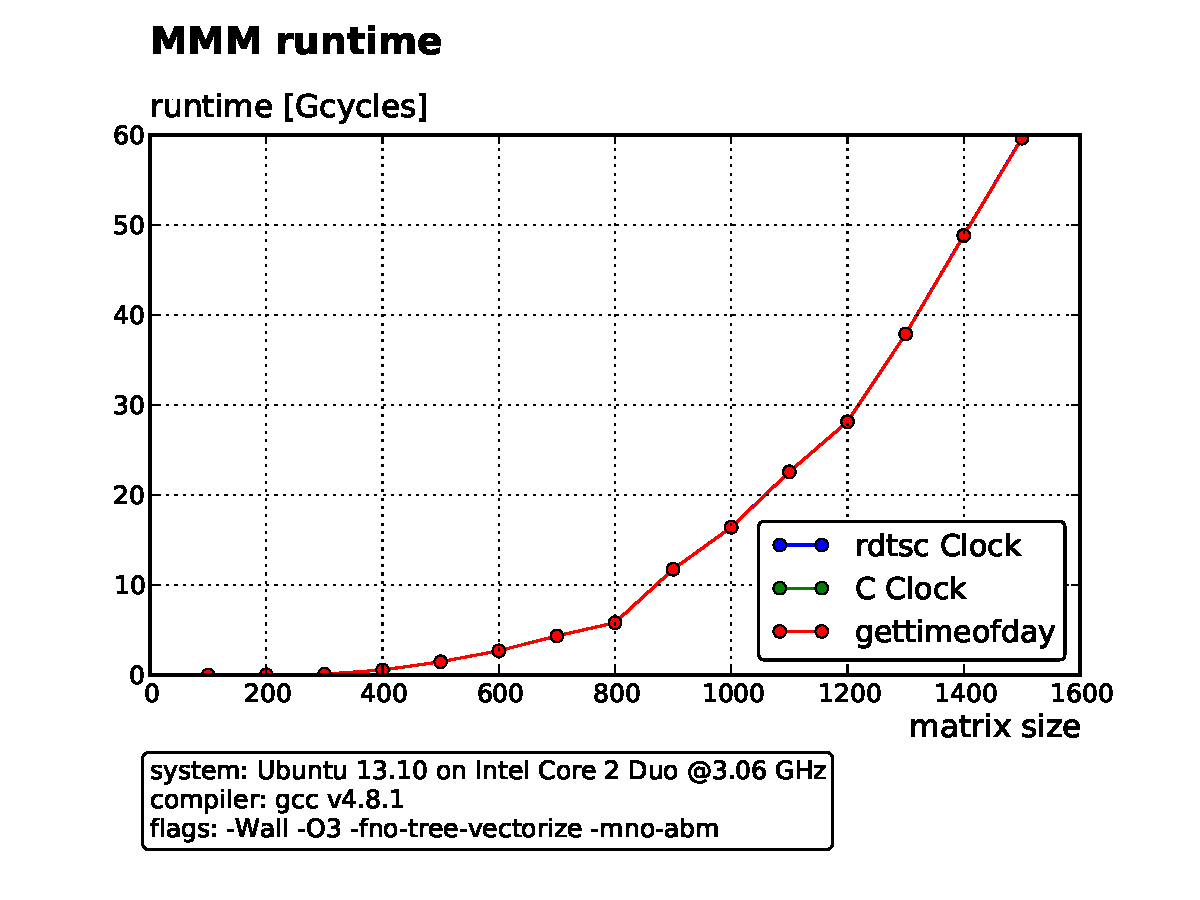
\includegraphics[width = 6in]{MMM_runtimeO3.pdf}
			\end{figure}
			\begin{figure}[H]
				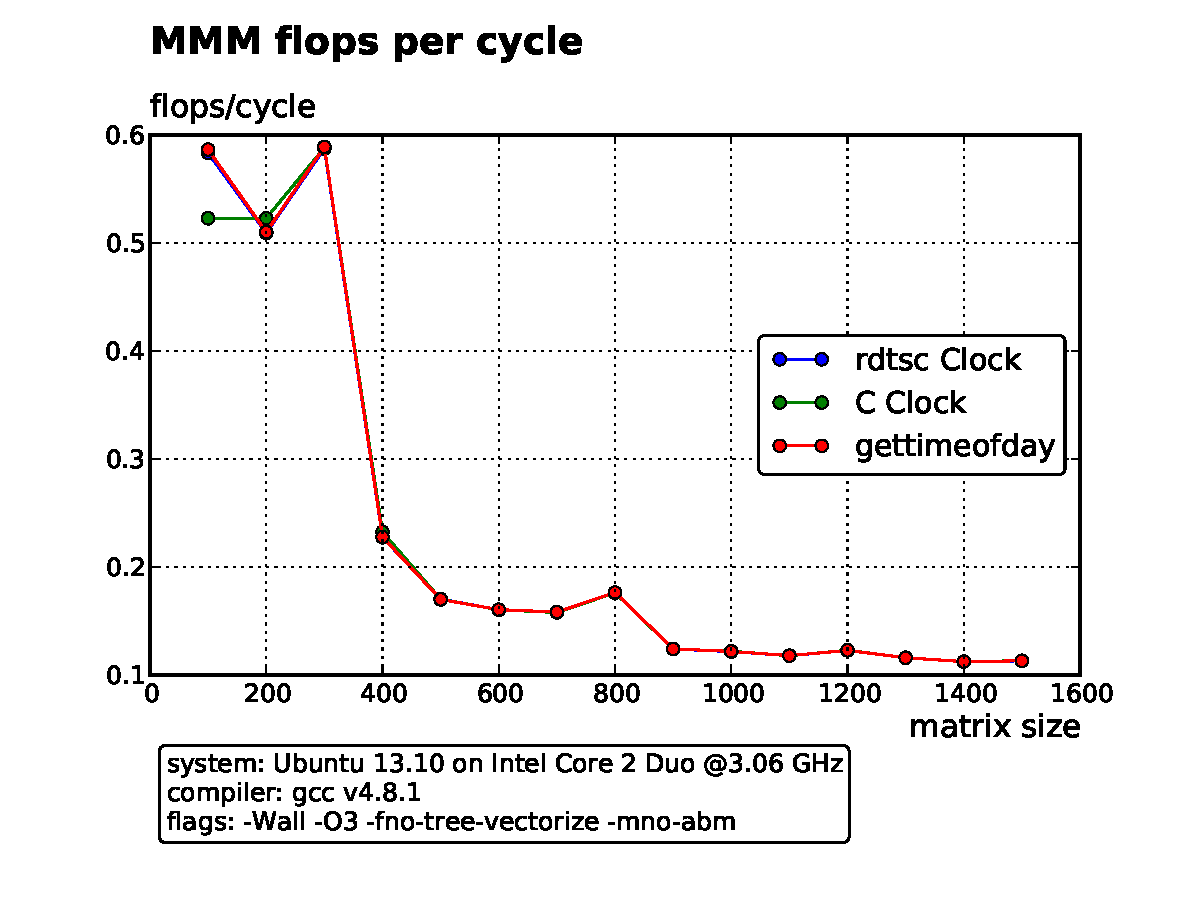
\includegraphics[width = 6in]{MMM_flopsO3.pdf}
			\end{figure}
			\begin{figure}[H]
				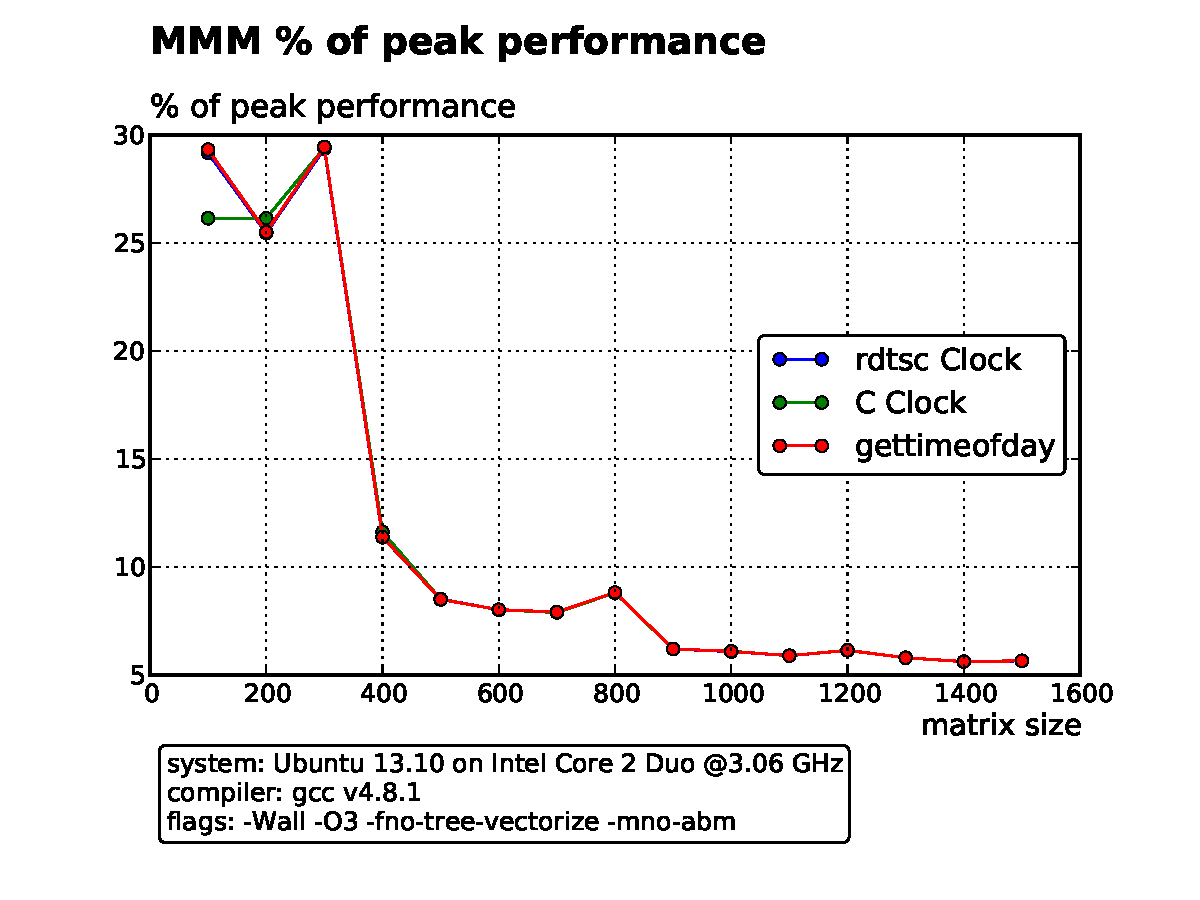
\includegraphics[width = 6in]{MMM_percentageO3.pdf}
			\end{figure}
	
	\section*{Exercise 4: MVM}
		\subsection*{a)} 
		I have used the exact structure from Ex. 3, but removed the other timing methods and changed the compute() function.\par 
		\emph{Remark: mvm.c can be found in $\mathtt{ex04/src/}$}
		\subsection*{b)}
		The compute() function uses:
		\[ m \cdot n \unit{add} + m \cdot n \unit{mult} = 2 \cdot m \cdot n \unit{flop} \]
		\subsection*{c)}
			\begin{figure}[H]
				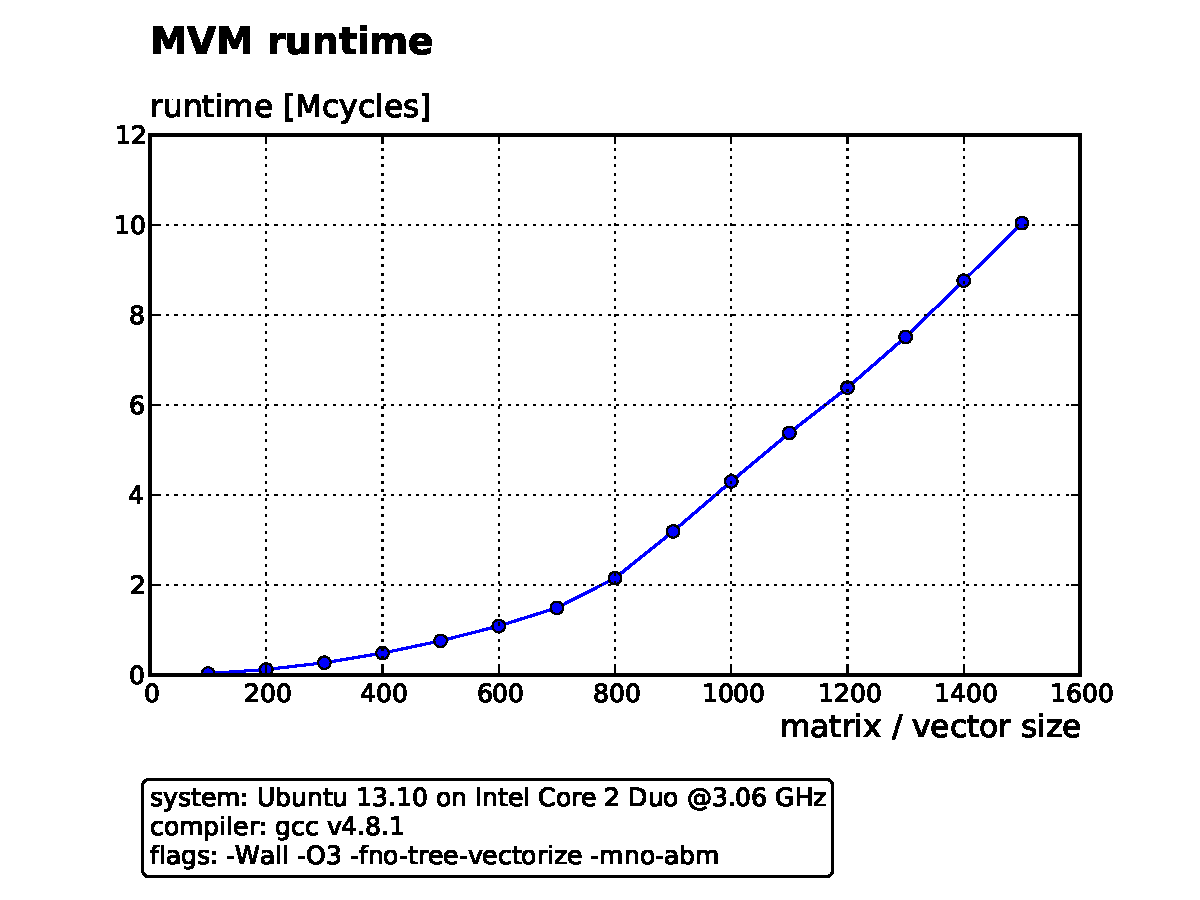
\includegraphics[width = 6in]{MVM_runtimeO3.pdf}
			\end{figure}
			\begin{figure}[H]
				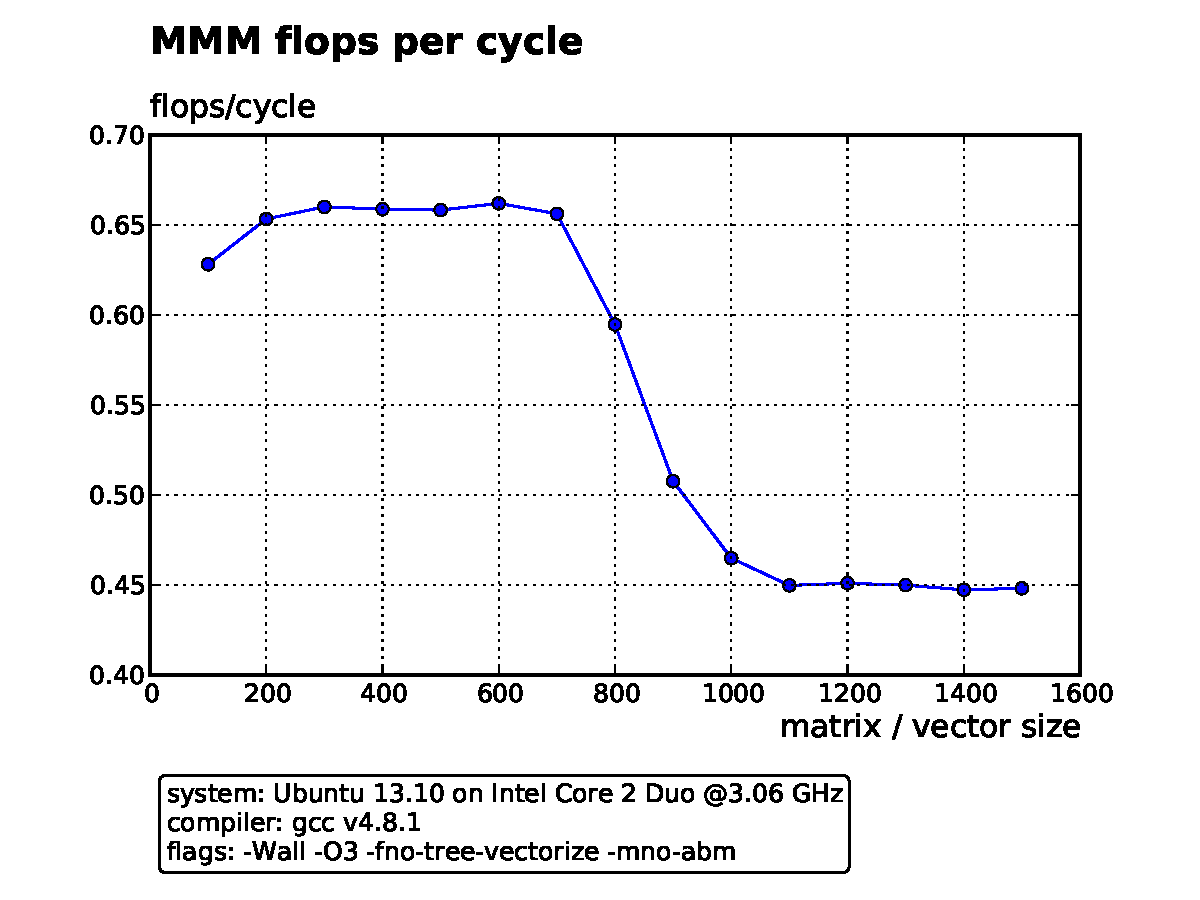
\includegraphics[width = 6in]{MVM_flopsO3.pdf}
			\end{figure}
			\begin{figure}[H]
				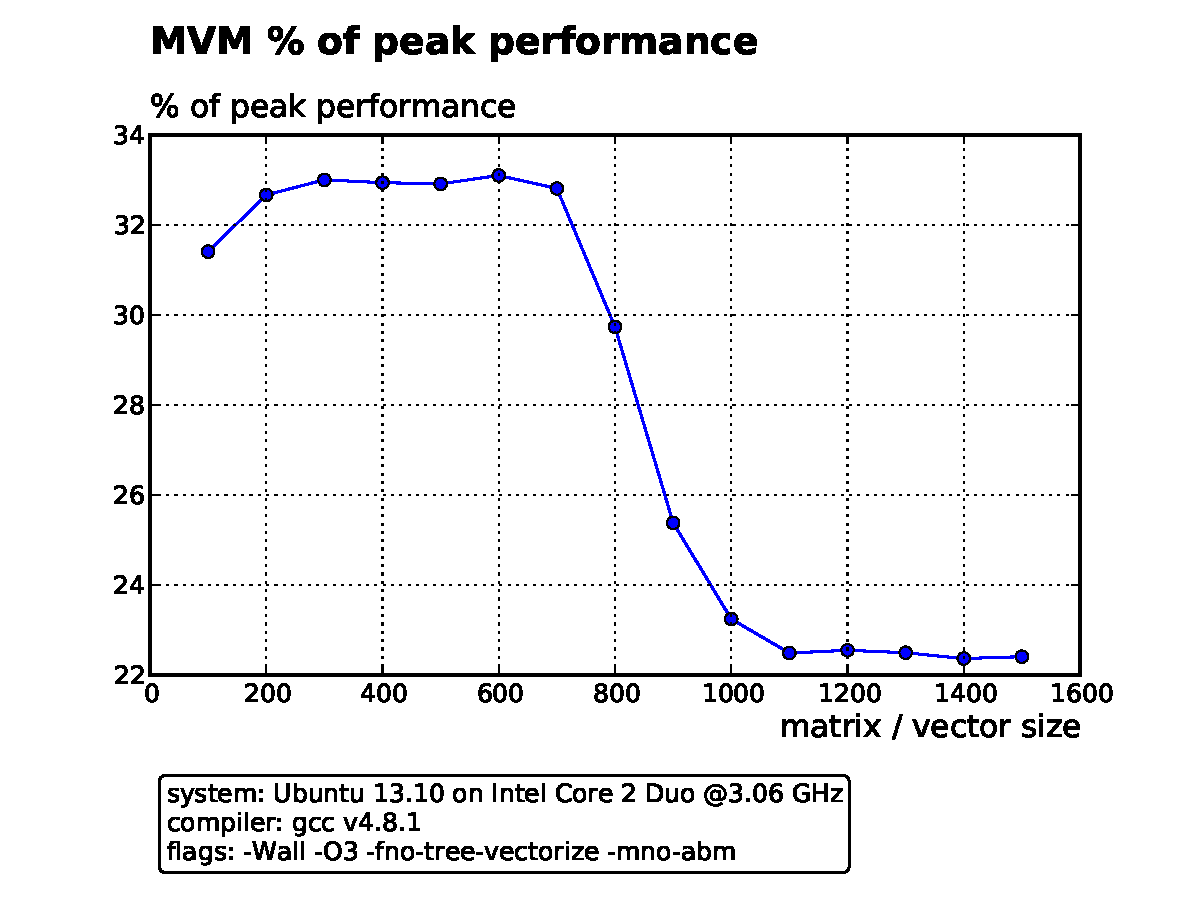
\includegraphics[width = 6in]{MVM_percentageO3.pdf}
			\end{figure}
		\section*{d)}
		At smaller $N$, both MMM and MVM start out at about $34 \%$ peak performance (both compiled at $\mathtt{-O3}$). The MVM, too, shows a dip in performance, but it is at much larger $N$ and the drop is less significant. This might be due to the fact that in the MVM compute() - function, the matrix (the part which - in memory size - is $N^3$) is accessed only once, and consecutively.
		
	\section*{Exercise 6: Bounds}
		\subsection*{a)}
			$9 \unit{mult}$ and $8 \unit{add}$ per innermost loop 
			$ \Rightarrow 17 \cdot (N - 1)^2 \unit{flop} = W(N) $
		\subsection*{b)}
			reads: $\geq N^2$ (size of G) $+ 9$ (size of h) $\unit{doubles} = 8 N^2 + 72 \unit{bytes}$ \\
			writes: $(N - 1)^2$ (one for each innermost loop) $ = 8(N - 1)^2 \unit{bytes}$ 
			\begin{align*}
				Q(N) =& 16 N^2 -16 N + 80 \unit{bytes}\\
				I(N) = & \frac{W(N)}{Q(N)} = \frac{17 (N - 1)^2}{16 N^2 -16 N + 80} \approx \frac{17}{16}
			\end{align*}
		the approximation is exact for large enough $N$.
		\subsection*{c)}
			\begin{itemize}
				\item[i)] Hard lower bound (not taking into account dependencies): \\\\
				for adds (latency: 3, throughput: 1): $8 \cdot (N-1)^2 + 2 \unit{cycles}$\\
				for mults (latency: 5, throughput: 1): $9 \cdot (N-1)^2 + 4 \unit{cycles}$ \\\\
				together: $\underline{9 \cdot (N-1)^2 + 4 \unit{cycles}}$ (limited by mults)
				\item[ii)] Numer of cycles used to load everything into memory for latency l and throughput tp (round up because you can only count full cycles):
				$\lceil \frac{Q(N) - 1}{tp} + l \rceil$\\\\
				in L1 (latency: 4, throughput: 4): $4 N^2 - 4 N + 24 \unit{cycles}$\\
				in L2 (latency: 12, throughput: 4): $4 N^2 - 4 N + 32 \unit{cycles}$\\
				in RAM (assuming latency: 100, throughput: 1/4): $64 N^2 - 64 N + 116 \unit{cycles}$
			\end{itemize}
\end{document}